\section{Principe de l'auralisation}

Nous allons nous intéresser dans ce projet uniquement à des salles en taille réelle avec une source et un récepteur
fixes. Dans ce cas particulier, la salle à étudier peut être assimilée à un filtre linéaire invariant par
translation dans le temps. 
Pour qu'un système puisse être considéré comme linéaire, il suffit que pour des entrées $x_1(t)$ et $x_2(t)$ et
leurs sorties respectives $y_1(t)$ et $y_2(t)$ on ait :

\begin{equation}
\alpha x_1(t) + \gamma x_2(t) \Leftrightarrow \alpha y_1(t) + \gamma y_2(t)
\end{equation}.
Dans notre cas, si 2 sons d'enveloppes et d'amplitude différentes sont émis dans une salle, il parait
logique ques ces sons n'interagiront pas entre eux et que par conséquent cette équation soit vérifiée dans
le cas de l'émission d'un son dans une salle avec un émetteur et recépteur fixes.
On peut dire qu'un système est invariant par translation dans le temps si, alors qu'à un temps $t$ une
entrée $x(t)$ est reliée à une sortie $y(t)$ on a pour un temps $t+\tau$ une entrée $x(t+\tau)$ liée à une
sortie $y(t+\tau)$ (voir figure~\ref{systeme_invariant}).

\begin{figure}[h!]
\begin{center}
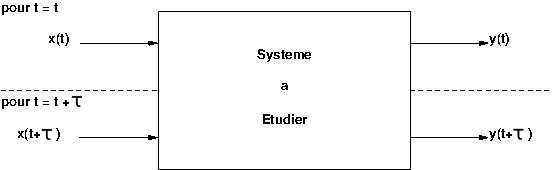
\includegraphics[width=10cm]{systeme_invariant.png}
\end{center}
\caption{\label{systeme_invariant} Le système à étudier est considéré invariant par translation dans le
temps si on peut lier les entrées aux sorties par une fonction de transfert immuable pendant le temps
considéré.}
\end{figure}

% De plus, un système peut être considéré comme invariant par translation dans le temps si pour une entrée
% $x_1(t)$ et une sortie $y_1(t)$ on a aussi, pour un intervale de temps $\tau$,  $x_1(t-\tau)$  qui correspond à
% $y_1(t-\tau)$.

Dans notre cas, à la condition que ni l'émetteur ni le récepteur ne change de position et que les conditions
extérieures ne fluctuent pas trop (température, pression ambiante), la réponse d'une salle à un son donné
n'a \textit{a priori} aucune raison de varier dans le temps.
Une salle peut donc bien être approximée à un système linéaire
On a donc le système présenté figure~\ref{systeme_lineaire_invariant}.

%%%%%% TODO %%%%%%%
% A complèter, à décommenter.
% Retirer ensuite les banières en commentaire

% \begin{figure}[h!]
% \begin{center}
% \includegraphics[width=10cm]{ NOM DE FICHIER}
% \end{center}
% \caption{\label{systeme_lineaire_invariant} LEGENDE }
% \end{figure}

%%%%%% END TODO %%%%%%%
